\section{Evaluation}

The following part of this work is not totally finished. Thus, some changes are
expected in the following days.

\subsection{Lean Scheduler}

As explained in earlier in this work, lean scheduler tries to achieve a shorter
job execution time by improving its load balancing. This is reflected by
achieving a smaller variance in task duration and more importantly at the task
ending time. Unfortunately, this perfect balance come with a cost, a very high
overhead to enable the proposed distributed lock systems and its communication.
\\ \\

As an iteration over the original ideal, there was the introduction of a new
technique which consisted in pre-assigning some percentage of the input while
leaving the remaining one free to be schedule by whatever task comes first.
This very technique has proven quite effective since our experiments shows that
Lean scheduler performs its best when we pre-assign most of the data, to be
more precise when we pre-assign from  $60\%$ to $80\%$ as shown in the
figure\ref{fig:lean_aggregate}.  \\

This does not come as a surprise, in fact reasons is that at an idle cluster we
have observed that tasks ending time variance was of about 20\% as shown at the
last figure of the grid \ref{fig:lean_grid}. In the very same figure we can see
how by pre-assigning less data, we get the less variable task duration while
incurring in a big overhead which determines a very big penalty at that job
execution time.

\begin{figure}[htbp]
\begin{tabular}{p{0.5\textwidth}p{0.5\textwidth}}
    \begin{minipage}{.5\textwidth}
    \centering
    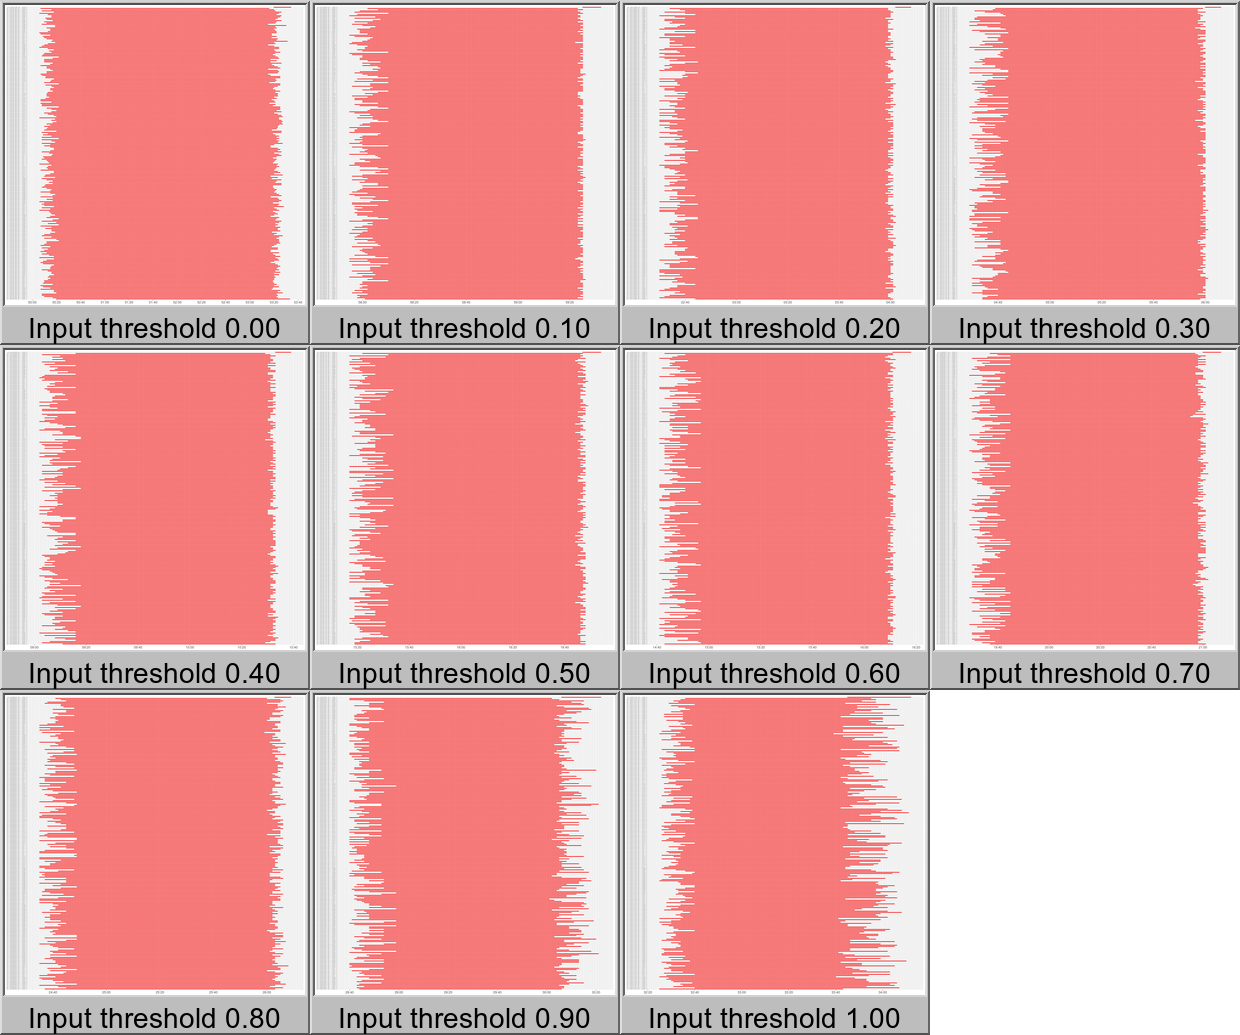
\includegraphics[width=1.0\textwidth]{figures/tasks_grid_small.png}
    \caption{IO monitoring architecture}
    \label{fig:lean_grid}
    \end{minipage}
    &
    \begin{minipage}{.5\textwidth}
    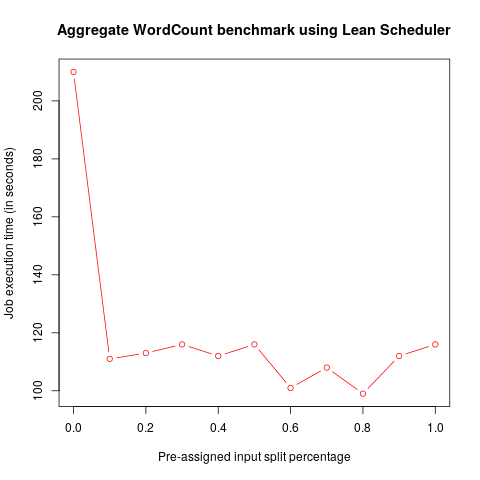
\includegraphics[width=1.0\textwidth]{figures/lean_aggregate.png}
    \caption{Lean Algorithm Aggregate wordcount}
    \label{fig:lean_aggregate}
    \end{minipage}
    \end{tabular}
\end{figure}

\subsection{IO aware scheduler and Recursive scheduler}

\subsection{Total comparison}
\lipsum[20]
